%%%%%%%%%%%%%%%%%%%%%%% file template.tex %%%%%%%%%%%%%%%%%%%%%%%%%
%
% This is a general template file for the LaTeX package SVJour3
% for Springer journals.          Springer Heidelberg 2010/09/16
%
% Copy it to a new file with a new name and use it as the basis
% for your article. Delete % signs as needed.
%
% This template includes a few options for different layouts and
% content for various journals. Please consult a previous issue of
% your journal as needed.
%
%%%%%%%%%%%%%%%%%%%%%%%%%%%%%%%%%%%%%%%%%%%%%%%%%%%%%%%%%%%%%%%%%%%

\RequirePackage{fix-cm}
%
%\documentclass{svjour3}                     % onecolumn (standard format)
%\documentclass[smallcondensed]{svjour3}     % onecolumn (ditto)
\documentclass[smallextended]{svjour3}       % onecolumn (second format)
%\documentclass[twocolumn]{svjour3}          % twocolumn
%

\smartqed  % flush right qed marks, e.g. at end of proof
%
\usepackage{graphicx}
\usepackage{natbib}
%
% \usepackage{mathptmx}      % use Times fonts if available on your TeX system
%
% insert here the call for the packages your document requires
%\usepackage{latexsym}
% etc.
%
% please place your own definitions here and don't use \def but
% \newcommand{}{}
%
% Insert the name of "your journal" with
\journalname{Attention, Perception, \& Psychophysics}
%
\begin{document}

\title{The effect of visualization on visual search performance
\thanks{}}

\subtitle{Does visualisation trump vision?}

\titlerunning{Does visualisation trump vision?}        % if too long for running head

\author{Alasdair D. F. Clarke, Courtney Barr  and  Amelia R. Hunt
}

%\authorrunning{Short form of author list} % if too long for running head

\institute{F. Author \at
              first address \\
              Tel.: +123-45-678910\\
              Fax: +123-45-678910\\
              \email{fauthor@example.com}           %  \\
%             \emph{Present address:} of F. Author  %  if needed
           \and
           S. Author \at
              second address
}

\date{Received: date / Accepted: date}
% The correct dates will be entered by the editor


\maketitle

\begin{abstract}
We propose a replication and generalisation of some striking results on the effect of mental imagery on visual search performance. 
\keywords{mental imagery \and visual attention, \and learning \and visual search \and perception \and open materials}
% \PACS{PACS code1 \and PACS code2 \and more}
% \subclass{MSC code1 \and MSC code2 \and more}
\end{abstract}

%%%%%%%%%%%%%%%%%%%%%%%%%%%%%%%%%%%%%%%%%%%%%%%%%%%%%
\section{Introduction}
\label{sec:intro}
%%%%%%%%%%%%%%%%%%%%%%%%%%%%%%%%%%%%%%%%%%%%%%%%%%%%%

Mental imagery is the term used to describe the representation of, or process of representing, an experience or activity in the absence of the represented sensory stimuli or behaviour. The processing mechanisms and experience of mental imagery of perceptual events can strongly resemble the experience of perceiving the actual external event. Indeed, many studies suggest mental imagery of perception is simply a weak form of perception (for a recent review, see \cite{pearson2015}). Consistent with this idea, imagining visual information (visualisation) can lead to classical conditioning \citep{lewis2013} and perceptual learning \citep{tartaglia2009}. This general framework dovetails with promising work suggesting that mental imagery can be a useful tool in clinical settings \citep[e.g.][]{foa1980} and in musical and athletic training \citep[e.g.][]{zatorre2007, guillot2008}. 

An interesting recent study by \cite{reinhart2015} demonstrated that attentional mechanisms can be effectively trained to select target objects through visualisation. Moreover, they found that visualising search for a particular target in an imagined array can speed reaction time to find the target on a subsequent trial even more than actually searching for the target in an array presented on the screen. In their experiments, participants were first shown a green C oriented in a particular direction, and then shown an array of 12 C's organized in a circle, only one of which was green. Participants had to press a key to indicate whether the one green C in the array was oriented in the same or a different direction as the C they had just been shown. Reaction times become faster when the C of a particular orientation repeated over a run of up to 7 trials. On some runs of trials participants were asked to "visualise search" and were shown the oriented C but not the array for the first two trials of the run. On trial 3 of the run, reaction time to find the target was significantly faster -- faster not only compared to the first trial of the run, but also faster when compared to trial 3 of runs during which the search array had actually been shown on trials 1 and 2. The authors also measured EEG during the experiment and found that the N2PC (an early component of stimulus-evoked EEG associated with attentional focus) followed a similar pattern as reaction time, with an enhanced N2PC to the third target in a run following two visualisation trials -- again, relative not only to the first trial in the run, but also to the third target following trials in which the search array was physically present rather than just visualised. The results suggest, as the title of the article states, that ``visalization trumps vision in training attention.'' 

On the one hand, this result is consistent with previous work reviewed above demonstrating that visualisation has meaningful effects on subsequent perception and behaviour. On the other, this result is unique in demonstrating that the effects of visualisation can surpass those of actual perception -- on its face, this is inconsistent with the idea that mental imagery is ``weak'' perception. One possible reason for the superiority of visualisation over perception, however, is that the perceptual learning over a run of trials when the target and distractors are displayed in fact has components of both interference and facilitation on the training of attention, and visualising removes some of the interference but maintains the facilitation. For example, the participant may may not imagine the distractors very vividly, and this could strengthen the representation of the target orientation, speeding reaction time to match it green C in the array on trial 3. Consistent with this interpretation, when the black distractor C's were removed from the display (Experiment 4), the difference between visualization and practice with actual stimuli was eliminated. This could reflect a floor effect, however, as reaction times in general in this experiment were much faster than in the experiments with distractors. It is also the case that the target can be rapidly selected on the basis of its color in this experiment, so processing of distractors would be expected to be minimal even when they are presented. If visualization was facilitated relative to search because the interference from distractors was minimised, even more facilitation for visualisation should be observed when search is difficult and the distractors during ``real'' search need to be processed in more detail. 

Definitively establishing why visualisation is more effective than actually performing the task is of critical importance not only for understanding the nature of visual imagery, but also because it could lead to improved imagery-based training or therapy regimes like those noted above. If it is the case that visualisation is more effective because it isolates the facilitative components of the task, for example, vague or incomplete representations may in fact be superior to less vivid or detailed ones. We therefore plan to first replicate the original study by \cite{reinhart2015}, focusing specifically on the behavioural results. Omitting the recording of EEG allows us to use a slightly simplified stimuli design to test the original results, without the second irrelevant coloured distractor (only included in the original study to allow for comparison of the lateralised N2PC component between the two hemifields). This will provide independent confirmation of this interesting result. We will also analyse the data in more depth using linear-mixed-effect models and explore how the visualisation effect changes over time and is affected by to serial dependencies \citep{fischer-whitney2014}. Provided we replicate the original findings, we also plan to run a second experiment using a more traditional visual search paradigm using an array of C's of uniform color, in which the observer's task is to determine whether the target (a C of the cued orientation) is present or absent. If the superiority of visualisation over practice at search is due to proactive interference from the distractors when the search array is presented, there should be even larger benefits of visualisation when serial search of all the items is required.  

%%%%%%%%%%%%%%%%%%%%%%%%%%%%%%%%%%%%%%%%%%%%%%%%%%%%%
\section{Experiment 1}
\label{sec:exp1}
%%%%%%%%%%%%%%%%%%%%%%%%%%%%%%%%%%%%%%%%%%%%%%%%%%%%%

The aim of this experiment is to directly replicate the behavioural effect of visualisation in visual search \citep{reinhart2015}. We have made two minor changes to the original paradigm: (i) we have removed the red distracter element used in the original study (included to measure the N2PC component of the EEG; we will not measure EEG). (ii). We will use runs of length three, four and five, rather than three, five and seven. This was done because 1) the practice effects asymptotes by trial 5 of the runs, and 2) runs of longer length are unimportant for testing the critical result: that reaction times for the first three trials in a run will be faster in the visualise condition than those in the practise condition. 

\subsection{Methods}

\subsubsection{Participants}

Thirty participants will be recruited via from amongst the student population at the University of Aberdeen. All participants will have normal or corrected-to-normal vision. 

The sample size of $n=30$ is based on a power analysis for a one-tailed paired $t$-test, with a power of 0.9 and effect size of $d=0.55$. This should be sufficient for the replication given the original effect sizes of $0.61<d<0.72$ ($n=18$).


\subsubsection{Stimuli}

The search stimuli consisted of twelve Landolt Cs arranged in a circle (radius $8^{\circ}$) around a central fixation cross. The Landolt C's had a radius of $0.62^{\circ}$ (with thickness $=0.25^{\circ}$, gap width$=0.19^{\circ}$) and had one of eight possible orientations ($\phi=n\frac{\pi}{4}$, $n=0,\ldots,7$). One of the C's was coloured green which indicated that it was the target. An example stimulus is shown in Fig. \ref{fig:exp1stimulus}.

\begin{figure}
\centering
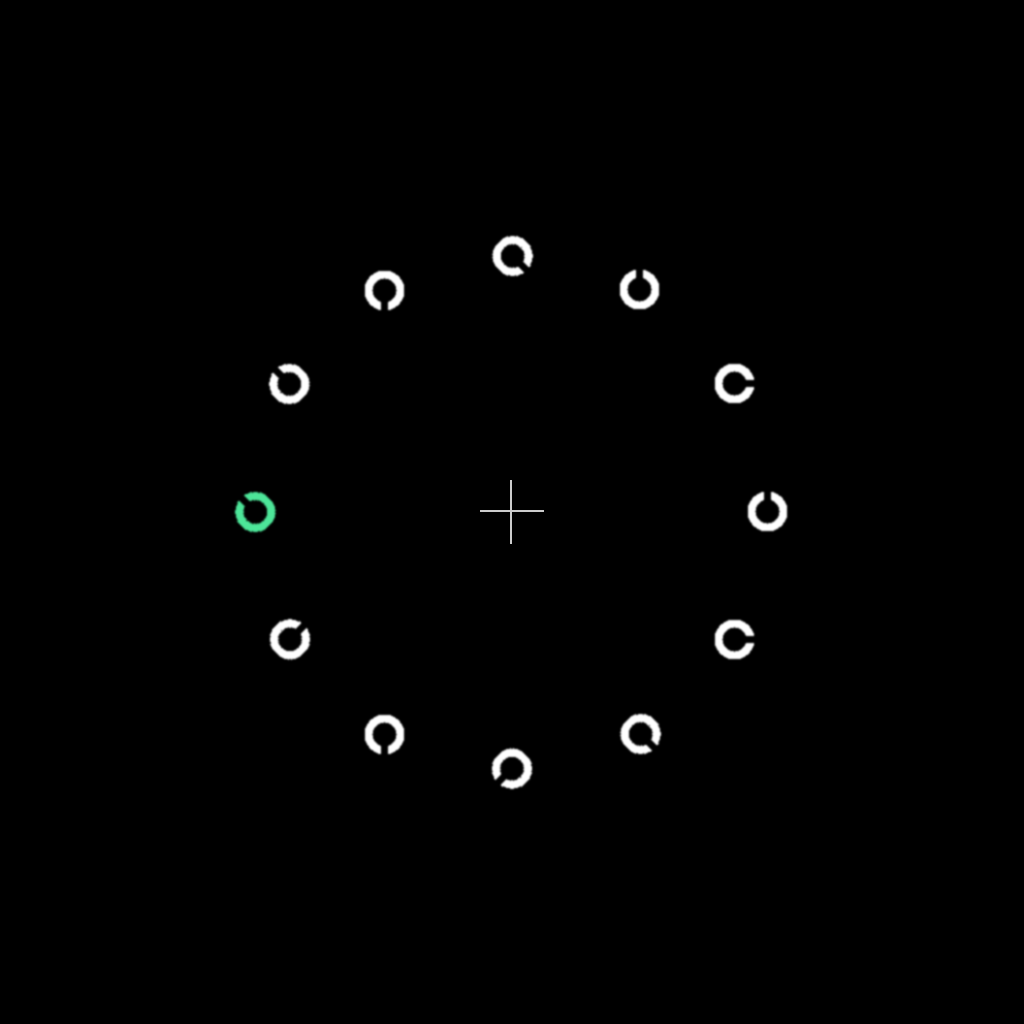
\includegraphics[width=6cm]{figs/exStimExp1.png}
\caption{Example stimulus from Experiment 1. Before the stimulus is shown, the observer is shown a green Landolt C. Their task is to decide if the green C in the stimulus matches the orientation of the cued C.}
\label{fig:exp1stimulus}
\end{figure}

\subsubsection{Procedure}
The first block of trials was pre-empted by a set of ten practice trials. The practice trials included the visual search condition only. There were then four blocks of 30 trials (15 for each condition). Each trial began with the presentation of a fixation cross (1200-1600ms) followed by the presentation of a green Landolt C (the cue stimuli) for 100ms, followed by a interval of 1000ms. The search array was then presented in the visual search condition for a maximum of 2000ms. In the visualise search condition the cue stimuli was followed by instructions to 'visualise search' before the presentation of a further fixation cross. The orientation of the green C, the location of the green C within the search array and whether the green C matched the cue was randomised for each trial.

\subsection{Planned Analyses}

We plan to carry out the analysis in several different ways. Firstly, we will repeat the analysis from \cite{reinhart2015} in which the median reaction time for trial 1,2 and 3 within a (normal) run is compared to the median reaction time for trial 3 in a visualise-run. A one-tailed paired $t$-test will be used for this comparison. We will include a Bayesian t-test which will enable comparison of the expected difference between visualisation and trials 1-3 in the run to the null hypothesis (no difference). We will also directly compare/combine our results with those of \cite{reinhart2015}, who have already provided us with the summary data from their Experiment 1. 

Additionally, we will also analyse our data in more detail using a linear mixed-effect model (\texttt{lme4} \citep{bates2015, R}), following the guidelines on model design given by \cite{barr2013} This allows us to include trial-to-trial variation in the analysis rather than using aggregate statistics. As the distribution of reaction times is expected to be skewed, we use log reaction times in the analysis. We will treat \textit{trial number} (within run) as a numerical factor, and will investigate non-linear regression if required (e.g. if there is a clear asymptote). However, given the results presented by \cite{reinhart2015}, a linear model should suffice. We will follow the model simplification procedure put forward by \cite[chapter 9]{crawley2012}. $p$-values will be obtained via the \texttt{Anova} function from the \texttt{car} package \citep{fox2011}.

Finally, we will also compare the visualisation effect to the effect of serial dependency. More specifically, we will investigate how reaction time varies on trial three depending on what preceded it (present-present, absent-absent, present-absent, absent-present, visualise-visualise). This will be modelled using another linear mixed-effect model with a five-level factor describing the previous two trials, and a two-level factor for whether trial three is a target absent or present trial.

\subsection{Results and Discussion}

\begin{center}
\textit{blank}
\end{center}

%%%%%%%%%%%%%%%%%%%%%%%%%%%%%%%%%%%%%%%%%%%%%%%%%%%%%
\section{Experiment 2}
\label{sec:exp2}
%%%%%%%%%%%%%%%%%%%%%%%%%%%%%%%%%%%%%%%%%%%%%%%%%%%%%

The aim of Experiment 2 is to investigate whether the effect reported by \cite{reinhart2015} applies to more standard visual search paradigms, or if it is specific to the target matching task they used in their original study. Hence, in this study we remove the colour cue from the stimuli and change the observer's task from `does the green item match the target template?' to `is the target present of absent in this stimulus?.' This study will only be run if we successfully replicate the visualisation effect in Experiment 1. 

\subsection{Methods}

Identical to Experiment 1, except the colour cue has been removed and participants report whether the target is present or absent. As this task is more difficult, stimulus display time (and the visualisation time) will be increased from 2000ms to 5000ms. 

\subsection{Results and Discussion}

\begin{center}
\textit{blank}
\end{center}

%%%%%%%%%%%%%%%%%%%%%%%%%%%%%%%%%%%%%%%%%%%%%%%%%%%%%
\section{General Discussion}
\label{sec:discussion}
%%%%%%%%%%%%%%%%%%%%%%%%%%%%%%%%%%%%%%%%%%%%%%%%%%%%%


\begin{center}
\textit{blank}
\end{center}


% BibTeX users please use one of
% \bibliographystyle{spbasic}      % basic style, author-year citations
%\bibliographystyle{spmpsci}      % mathematics and physical sciences
%\bibliographystyle{spphys}       % APS-like style for physics

\bibliographystyle{plainnat}
\bibliography{literature}

\end{document}
% end of file template.tex

